\section{표본분포}
모집단 전체를 조사하는 것은 비용이 많이 들고, 또 현실적으로 어렵다. 따라서 통계적 추정을 할 때에는 표본을 뽑아 조사하는 것이 경제적이다.\\

\defn{모집단에서 임의추출한 표본으로부터 얻은 통계량은 확률변수이므로 분포를 가지게 된다. 이를 \textbf{표본분포}(sampling distribution)라 한다.}

\defn{모집단에서 임의추출한 크기 $n$인 표본을 $X_1, \dots, X_n$ 이라 할 때,
\begin{itemize}
	\item \textbf{표본평균}(sample mean): $\overline{X} = \ds \frac{1}{n}\sum_{i=1}^n X_i$
	\item \textbf{표본분산}: $S^2 = \ds \frac{1}{n-1}\sum_{i=1}^n \left(X_i-\overline{X}\right)^2$
\end{itemize}
표본을 뽑을 때마다 표본평균, 표본분산은 달라질 수 있으므로 $\overline{X}, S^2$은 확률변수가 된다. 따라서, 기댓값, 분산, 표준편차도 계산할 수 있다.
}

\prob{모집단 $\{1, 3, 5, 7\}$ 에서 크기가 2인 표본을 복원추출 할 때, 표본평균 $\overline{X}$의 확률분포가 다음과 같다.
\begin{center}
	\begin{tabular}{c|c|c|c|c|c|c|c|c}
		$\overline{X}$ & 1&2&3&4&5&6&7&합계\\\hline
		$\pr(\overline{X} = \overline{x})$ & $\frac{1}{16}$ & $\frac{1}{8}$ & $a$ & $b$ & $\frac{3}{16}$ & $c$ & $\frac{1}{16}$ &1
		
	\end{tabular}
\end{center}
이 때, $a, b, c$ 의 값을 구하고, 확률변수 $\overline{X}$의 기댓값과 분산을 구하여라.}\\

\defn{$X_i$ 를 $i$-번째로 뽑힌 추출단위의 특성값을 나타내는 확률변수라 하자. 다음 조건을 만족하는 $X_1, \dots, X_n$ 을 \textbf{랜덤표본}(random sample)이라 한다.
\begin{enumerate}
	\item[(1)] (유한모집단) 단순랜덤 비복원추출로 뽑은 표본
	\item[(2)] (무한모집단) $X_i$ 들은 서로 독립이고 각 분포가 모집단 분포와 동일
\end{enumerate}
참고: 유한모집단에서 모집단의 크기가 큰 경우에는 흔히 무한모집단에서의 랜덤표본으로 간주하여 표본분포를 구한 다음 이를 실제표본분포의 근사분포로 사용한다.
}

\thm{모평균이 $\mu$이고 모표준편차가 $\sigma$인 모집단에서\footnote{무한모집단의 경우 복원추출이나 비복원추출이나 큰 차이가 없다.} 복원추출하여 뽑은 크기가 $n$인 표본의 표본평균 $\overline{X}$에 대하여 다음이 성립한다. $$\ex(\overline{X}) = \mu, \: \var(\overline{X}) = \frac{\sigma^2}{n}, \: \sigma(\overline{X}) = \frac{\sigma}{\sqrt{n}}$$
\textbf{증명}. $\overline{X} = \ds \frac{1}{n} \sum_{i=1}^n X_i$ 를 이용한다.\\
$$\ex(\overline{X}) = \ds \frac{1}{n}\ex(X_1+\cdots + X_n) = \frac{n\mu}{n} = \mu$$$$\var(\overline{X}) =\ds \frac{1}{n^2}\var(X_1+\cdots+X_n) = \frac{1}{n^2}\sum_{i=1}^n \var(X_i) = \frac{n\sigma^2}{n^2} = \frac{\sigma^2}{n}$$ \qed\\
\textbf{참고}: 모평균이 $\mu$, 모분산이 $\sigma^2$, 크기가 $N$인 유한모집단에서 크기 $n$인 표본을 비복원추출하는 경우에는 다음이 성립한다. $$\ex(\overline{X}) = \mu, \: \var(\overline{X}) = \frac{N-n}{N-1}\cdot\frac{\sigma^2}{n}$$
여기서 $\sqrt{\frac{N-n}{N-1}}$ 은 finite-population correction factor (FPC) 로 불린다.
}


\prob{연습문제 9.3 에서 구한 $\overline{X}$ 의 기댓값과 분산이 위 정리를 사용하여 구한 것과 일치함을 확인하여라.}

\thm{표본의 크기가 클수록 표본평균과 모평균의 오차가 줄어든다.}

\thm{모집단의 분포가 $\mc{N}(\mu, \sigma^2)$ 일 때, 표본평균 $\overline{X}$는 $\mc{N}(\mu, \sigma^2/n)$ 을 따른다.}

\prob{$\mc{N}(100, 2^2)$ 을 따르는 모집단에서 크기가 4인 표본을 임의추출할 때, 표본평균 $\overline{X}$가 따르는 분포를 구하여라.}

\prob{어느 전기 회사에서 생산하는 전구의 수명을 나타내는 확률변수 $X$에 대하여, $X\sim \mc{N}(2000, 200^2)$ 이라고 한다. 이 회사가 생산한 전구 중 임의추출한 $n$개 전구의 평균 수명을 $\overline{X}$라 할 때, $\pr(1900 \leq \overline{X}\leq 2100)\geq0.9$ 가 성립하기 위한 $n$의 최솟값을 구하여라. 단, $z_{0.05} = 1.65$ 이다.}

\thm{(\textbf{중심극한정리} - Central Limit Theorem) 평균이 $\mu$이고 분산이 $\sigma^2$인 임의의 무한모집단에서 표본의 크기 $n$이 충분히 크면, 랜덤표본의 표본평균 $\overline{X}$는 근사적으로 정규분포 $\mc{N}\left(\mu, \ds \frac{\sigma^2}{n}\right)$ 을 따른다.\footnote{당연히, $n$이 클수록 근사는 정확해진다.}}

\prob{대학 신입생 신장의 평균이 168cm이고 표준편차가 6cm임이 알려져 있다. 100명의 신입생을 단순랜덤추출하는 경우 표본평균이 167cm 이상 169cm 이하일 확률을 구하여라. 단, $z_{0.0475} = 1.67$ 이다.}\\\\

\defn{확률변수 $Z_1, \dots, Z_k$ 이 $\mc{N}(0, 1)$의 랜덤표본일 때, $V = Z_1^2+\cdots+Z_k^2$ 의 분포를 \textbf{자유도}(degrees of freedom) $k$인 \textbf{카이제곱분포}($\chi^2$-distribution)라고 한다. 기호로는 다음과 같이 나타낸다. $$Z_1^2+\cdots+Z_k^2 = V \sim \chi^2(k)$$그리고 확률밀도함수는 다음과 같다.\footnote{$\Gamma$ 는 감마함수(Gamma function)을 나타내는 기호이다.} $$\frac{1}{2^{k/2}\Gamma(k/2)}x^{k/2-1}e^{-x/2} \qquad (x > 0)$$}

\begin{center}
	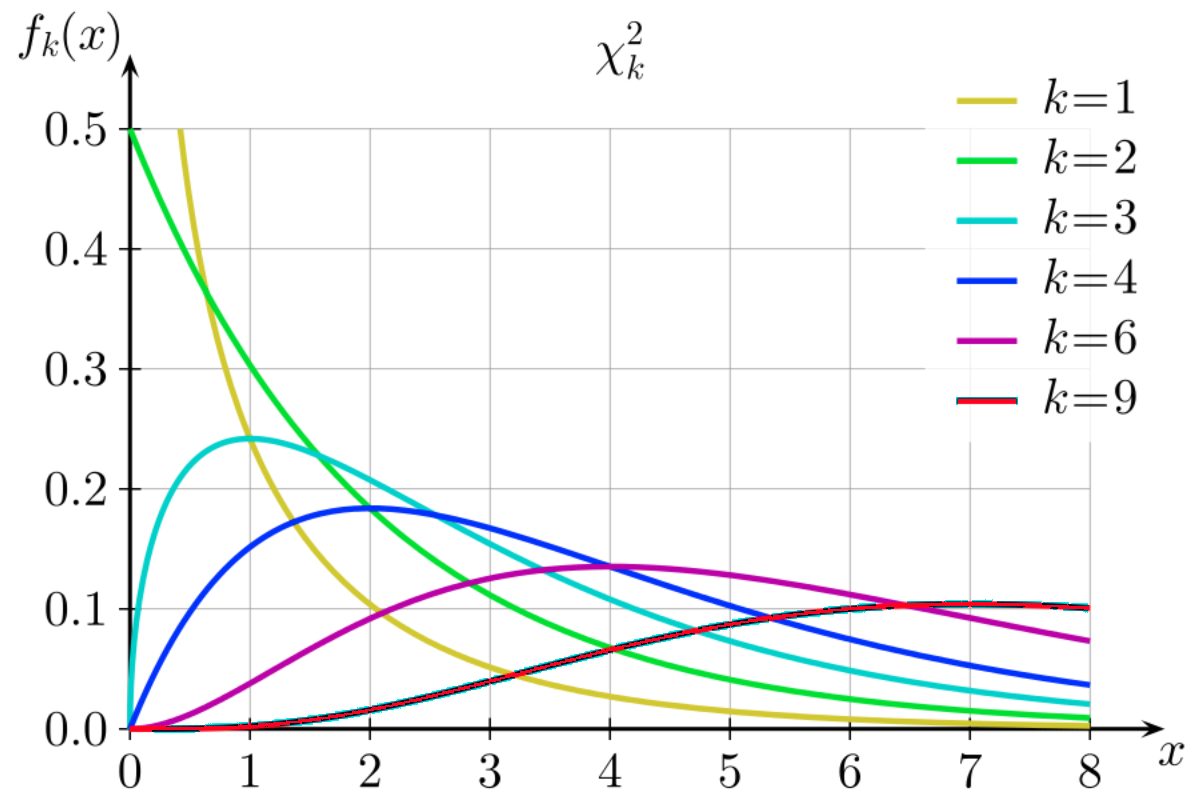
\includegraphics[width=10.098cm, height=8cm]{chisq.png}\\
	$\chi^2$-분포의 형태 ($k$: 자유도)
\end{center}

\defn{$V\sim \chi^2(k)$ 일 때, $\pr(V>v)=\alpha$ 인 $v$의 값을 $\chi^2_\alpha(k)$ 로 정의한다.}

\thm{(카이제곱분포의 가법성) $V_1, V_2$가 서로 독립이면 다음이 성립한다.
\begin{enumerate}
	\item[(1)] $V_1\sim \chisq(k_1)$, $V_2\sim \chisq(k_2)$ 이면 $V_1+V_2 \sim \chisq(k_1+k_2)$
	\item[(2)] $V_1\sim \chisq(k_1)$, $V_1+V_2\sim \chisq(k_1+k_2)$ 이면 $V_2\sim \chisq(k_2)$
\end{enumerate}}

\thm{$X_1, \dots, X_n$이 $\mc{N}(\mu, \sigma^2)$의 랜덤표본일 때, 표본분산 $S^2 = \ds \frac{1}{n-1}\sum_{i=1}^n (X_i-\overline{X})^2$ 에 대하여 다음이 성립한다. $$\frac{(n-1)S^2}{\sigma^2} \sim \chisq(n-1)$$ 
\textbf{증명}. 모든 $i$에 대해 $\dfrac{X_i-\mu}{\sigma} \sim \mc{N}(0, 1)$ 이고 서로 독립이므로 카이제곱분포의 정의로부터
$$\sum_{i=1}^n \left(\frac{X_i-\mu}{\sigma}\right)^2 \sim \chisq(n)$$
이 성립한다. 그런데, 표본분산 $S^2$의 정의로부터
$$\sum_{i=1}^n \left(\frac{X_i-\mu}{\sigma}\right)^2 = \sum_{i=1}^n \left(\frac{X_i-\overline{X}}{\sigma}\right)^2 + n\left(\frac{\overline{X}-\mu}{\sigma}\right)^2 = \frac{(n-1)S^2}{\sigma^2} + \left(\frac{\overline{X}-\mu}{\sigma/\sqrt{n}}\right)^2$$
이고 $\ds \left(\frac{\overline{X}-\mu}{\sigma/\sqrt{n}}\right)^2 \sim \chisq(1)$ 이므로 가법성에 의해 $\ds \frac{(n-1)S^2}{\sigma^2} \sim \chisq(n-1)$.\qed
}

\thm{분산이 동일한 두 정규모집단 $\mc{N}(\mu_1, \sigma^2)$, $\mc{N}(\mu_2, \sigma^2)$ 에서 각각 뽑은 랜덤표본 $X_1, \dots, X_{n_1}$ 과 $Y_1, \dots, Y_{n_2}$ 이 서로 독립이라고 하자. $S_1^2, S_2^2$를 각각 $X_i, Y_i$ 의 표본분산이라 할 때, \textbf{합동표본분산}(pooled sample variance) $$S_p^2 = \frac{(n_1-1)S_1^2 +(n_2-1)S_2^2}{n_1+n_2-2}$$에 대하여 다음이 성립한다. $$\frac{(n_1+n_2-2)S_p^2}{\sigma^2} \sim \chisq (n_1+n_2-2)$$
\textbf{증명}. 다음을 이용하면 가법정리에 의해 자명하다. $$S_p^2 = \frac{(n_1-1)}{(n_1-1)+(n_2-1)} S_1^2+\frac{(n_2-1)}{(n_1-1)+(n_2-1)} S_2^2$$\qed}

\defn{$Z\sim \mc{N}(0, 1)$ 과 이와 독립인 확률변수 $V$가 자유도가 $k$인 카이제곱분포를 따를 때, $T=\dfrac{Z}{\sqrt{V/k}}$ 의 분포를 자유도가 $k$인 \textbf{$t$-분포}($t$-distribution)라 한다.\footnote{스튜던트의(Student's) $t$-분포 라고 불리기도 한다.} 기호로는 다음과 같이 나타낸다. $$\frac{Z}{\sqrt{V/k}} = T \sim t(k)$$그리고 확률밀도함수는 다음과 같다. 
	$$\frac{\Gamma\left(\frac{k+1}{2}\right)}{\sqrt{k\pi}\,\Gamma\left(\frac{k}{2}\right)}\left(1+\frac{x^2}{k}\right)^{-\frac{k+1}{2}} \qquad (-\infty < x <\infty)$$
}
\begin{center}
	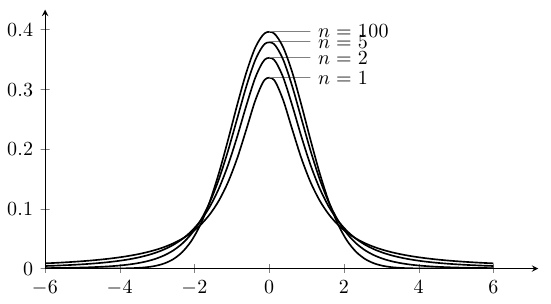
\includegraphics[width=9.0625cm, height=5cm]{tdist}\\
	$t$-분포의 형태 ($n$: 자유도)
\end{center}

\thm{$t$-분포 곡선은 0을 중심으로 좌우 대칭의 밀도곡선을 가지며, 자유도 $k$가 커지면 $\mc{N}(0, 1)$과 비슷하며, 일반적으로 표준정규분포보다 더 두꺼운 꼬리를 갖고 있다.}

\defn{$T\sim t(k)$ 일 때, $\pr(T>t)=\alpha$ 인 $t$의 값을 $t_\alpha(k)$ 로 정의한다.}

\thm{$X_1, \dots, X_n$ 이 $\mc{N}(\mu, \sigma^2)$의 랜덤표본일 때, 다음이 성립한다. $$\frac{\overline{X}-\mu}{S/\sqrt{n}}\sim t(n-1)$$
\textbf{증명}. 다음 변형을 이용한다.
$$\frac{\overline{X}-\mu}{S/\sqrt{n}} = \frac{\left(\overline{X}-\mu\right) / \left(\dfrac{\sigma}{\sqrt{n}}\right)}{\sqrt{\dfrac{(n-1)S^2}{\sigma^2}/ (n-1)}}$$
$\ds \frac{\overline{X}-\mu}{\sigma/\sqrt{n}} \sim \mc{N}(0, 1)$ 이고, $\dfrac{(n-1)S^2}{\sigma^2} \sim \chisq(n-1)$ 이며, $\overline{X}$ 와 $S^2$은 서로 독립임이 알려져 있다. $t$-분포의 정의에 의해 성립한다.\qed
}

\thm{분산이 동일한 두 정규모집단 $\mc{N}(\mu_1, \sigma^2)$, $\mc{N}(\mu_2, \sigma^2)$ 에서 각각 뽑은 랜덤표본 $X_1, \dots, X_{n_1}$ 과 $Y_1, \dots, Y_{n_2}$ 이 서로 독립이라고 하자. $X_i, Y_i$ 의 표본분산 $S_1^2, S_2^2$, 합동표본분산 $S_p^2$에 대하여 다음이 성립한다. $$\frac{(\overline{X}-\overline{Y}) - (\mu_1-\mu_2)}{S_p \sqrt{\dfrac{1}{n_1}+\dfrac{1}{n_2}}} \sim t(n_1+n_2-2)$$
\textbf{증명}. 다음 변형을 이용한다.
$$\frac{(\overline{X}-\overline{Y}) - (\mu_1-\mu_2)}{S_p \sqrt{\dfrac{1}{n_1}+\dfrac{1}{n_2}}} = \frac{\left[(\overline{X}-\overline{Y}) - (\mu_1-\mu_2)\right] / \left(\sigma \sqrt{\dfrac{1}{n_1} + \dfrac{1}{n_2}}\right)}{\sqrt{\dfrac{(n_1+n_2-2)S_p^2}{\sigma^2}/(n_1+n_2-2)}}$$
분모는 $\mc{N}(0, 1)$ 을 따르고, 정리 9.17에 의해 $t$-분포의 정의를 만족한다. \qed
}

\defn{$V_1\sim \chisq(k_1)$, $V_2\sim \chisq(k_2)$ 이고 $V_1, V_2$가 서로 독립일 때, $$F=\frac{V_1/k_1}{V_2/k_2}$$ 의 분포를 자유도 $(k_1, k_2)$ 인 $F$-분포라고 한다. 기호로는 다음과 같이 나타낸다.$$\frac{V_1/k_1}{V_2/k_2}=F\sim F(k_1, k_2)$$
그리고 확률밀도함수는 다음과 같다.\footnote{B 는 베타함수(Beta function)을 나타낸다.}
$$\frac{\sqrt{\dfrac{(k_1x)^{k_1}k_2^{k_2}}{(k_1x+k_2)^{k_1+k_2}}}}{x\mr{B}\left(\dfrac{k_1}{2}, \dfrac{k_2}{2}\right)} \qquad (x > 0)$$}

\defn{$F\sim F(k_1, k_2)$ 일 때, $\pr(F>f)=\alpha$ 인 $f$의 값을 $F_\alpha(k_1, k_2)$ 로 정의한다.}

\thm{~
\begin{enumerate}
	\item[(1)] $F\sim F(k_1, k_2)$ 이면, $1/F \sim F(k_2, k_1)$ 이다.
	\item[(2)] $F_{1-\alpha}(k_2, k_1) = 1/F_\alpha(k_1, k_2)$
	\item[(3)] $T\sim t(k)$ $\iff$ $T^2 \sim F(1, k)$
\end{enumerate}
}

\thm{두 정규모집단 $\mc{N}(\mu_1, \sigma_1^2)$, $\mc{N}(\mu_2, \sigma_2^2)$ 에서 각각 뽑은 랜덤표본 $X_1, \dots, X_{n_1}$ 과 $Y_1, \dots, Y_{n_2}$ 이 서로 독립이라고 하자. $X_i, Y_i$ 의 표본분산 $S_1^2, S_2^2$에 대하여 다음이 성립한다.
$$\frac{S_1^2/\sigma_1^2}{S_2^2/\sigma_2^2} \sim F(n_1-1, n_2-1)$$
\textbf{증명}. 다음과 같이 변형한다.
$$\frac{S_1^2/\sigma_1^2}{S_2^2/\sigma_2^2} = \frac{\dfrac{(n_1-1)S_1^2}{\sigma_1^2}/(n_1-1)}{\dfrac{(n_2-2)S_2^2}{\sigma_2^2}/(n_2-1)}$$
$\dfrac{(n_1-1)S_1^2}{\sigma_1^2} \sim \chisq(n_1-1)$, $\dfrac{(n_2-2)S_2^2}{\sigma_2^2}\sim \chisq(n_2-1)$ 이므로 $F$-분포의 정의를 만족한다. \qed 
}

\pagebreak